\documentclass[review]{elsarticle}
\biboptions{numbers,sort&compress}
\usepackage{lineno}
\usepackage{xspace}
\usepackage[T1]{fontenc}
\usepackage{lmodern}
\modulolinenumbers[5]

\journal{Applied Energy}

%% `Elsevier LaTeX' style

%%%%%%%%%%%%%%%%%%%%%%%

%%%% packages and definitions (optional)
\usepackage{placeins}
\usepackage{footnote}
%\makesavenoteenv{tabularx}
\usepackage{booktabs} % nice rules (thick lines) for tables
\usepackage{longtable} % for 'longtable' environment
\usepackage{pdflscape} % for 'landscape' environment
\usepackage{microtype} % improves typography for PDF
\usepackage{hhline}
\usepackage{amsmath}
\usepackage{pifont}
\usepackage{mathrsfs}
\usepackage{rotating}
\usepackage{tablefootnote}
\usepackage{multirow}
\usepackage{longtable}
\usepackage{enumitem}
\usepackage{mathtools}
\usepackage{amssymb}
\usepackage{float}
\usepackage{footnote}
\usepackage{slashbox}
\newcommand{\abs}[1]{\left\lvert #1 \right\rvert}
%\usepackage{adjustbox}
%\usepackage{cite}
%\usepackage[demo]{graphicx}
%\usepackage{caption}
%\usepackage{subcaption}

\usepackage{booktabs}
\usepackage{threeparttable, tablefootnote}

\usepackage{tabularx}
\newcolumntype{b}{>{\hsize=1.0\hsize}X}
\newcolumntype{s}{>{\hsize=.5\hsize}X}
\newcolumntype{m}{>{\hsize=.75\hsize}X}
\newcolumntype{x}{>{\hsize=.25\hsize}X}

\graphicspath{{figures/}}

% tikz %
\usepackage{tikz}
\usepackage{chronology}
\usetikzlibrary{arrows.meta}

\usetikzlibrary{positioning, arrows, decorations, shapes, calc }
% Define block styles
\tikzstyle{decision} = [diamond, draw, fill=blue!20, 
text width=4.5em, text badly centered, node distance=3cm, inner sep=0pt]

\tikzstyle{const} = [rectangle, draw, text centered, fill=orange!20]
\tikzstyle{data} = [rectangle, draw, text centered, fill=green!20]

\tikzstyle{block} = [rectangle, draw, text centered, fill=blue!20]
\tikzstyle{line} = [draw, -latex']
\tikzstyle{cloud} = [draw, ellipse,fill=red!20, node distance=6em,
minimum height=2em]



\usetikzlibrary{shapes.multipart}
\usetikzlibrary{positioning}
% hyperref %
\usepackage[hidelinks]{hyperref}
% after hyperref %
\usepackage{cleveref}
\usepackage{datatool}
%\usepackage[nonumberlist,nopostdot,nonumberlist,acronym,toc,section]{glossaries}
\usepackage[xindy,nonumberlist]{glossaries}
\newacronym{<++>}{<++>}{<++>}
\newacronym{I$^2$CNER}{I$^2$CNER}{International Institute for Carbon Neutral Energy Research}
\newacronym{MARKAL}{MARKAL}{MARKet ALlocation}
\newacronym{TIMES}{TIMES}{The Integrated MARKAL-EFOM System}
%\newacronym[longplural={metric tons of heavy metal}]{MTHM}{MTHM}{metric ton of heavy metal}


\makeglossaries

\newcommand{\greencheck}{{\color{green}\checkmark}}
\newcommand{\xmark}{{\color{red}\ding{55}}}
\usepackage[includefoot,bottom=8pt]{geometry}



\begin{document}
\begin{frontmatter}
\title{The role of current and emerging technologies in meeting Japan's mid- to long-term carbon reduction goals}

\date{}                     %% if you don't need date to appear

%% Authors
\author[uiuc]{Anshuman Chaube\corref{corrauthor}}
\cortext[corrauthor]{Corresponding Author}
\ead{achaube2@illinois.edu}
\author[ku]{Andrew Chapman}
\author[uiuc]{James Stubbins}
\author[uiuc]{Kathryn D. Huff} %



% Institutes of the authors
\address[uiuc]{Department of Nuclear, Plasma, and Radiological Engineering, University of Illinois at Urbana-Champaign, Urbana, IL 61801, United States}
\address[kuead]{Multiscale Science and Engineering for Energy and the Environment, International Institute for Carbon-Neutral Energy Research, Kyushu University, 744 Motooka, Nishi-ku, Fukuoka 819-0395, Japan.}
\address[kumech]{Department of Mechanical Engineering, Kyushu University,744 Motooka, Nishi-ku, Fukuoka 819-0395, Japan.}

	
\begin{keyword}
%insert keywords here
energy model \sep
Japan \sep
hydrogen fuel cell \sep
nuclear power \sep
carbon capture
\end{keyword}


\begin{abstract}

We simulated possible pathways to meeting 2030 and 2050 emission targets within the Japanese electricity supply sector using a single-region \gls{TIMES} model. Key features of our simulations include the incorporation of novel technologies, like hydrogen electrolysers, carbon capture, photochemical water splitting, and emerging photovoltaic cells, long-term impact assessment up to the year 2100, the inclusion of life-cycle emission and learning curves for technology costs and emission coefficients. Results indicate that a hybrid approach, using nuclear power and hydrogen from renewable energy-based electrolysis, is cost-effective and provides long-term emission reduction along with energy security. Nuclear, wind, solar, and hydrogen from renewables emerge as key emission reduction technologies, while natural gas with carbon capture plays a minor role.

\end{abstract}

\end{frontmatter}
%\glsresetall
\glsaddall

\linenumbers

\printglossary[title=Abbreviations]

\section{Introduction} \label{Introduction}
In order to mitigate climate change and to improve environmental outcomes, many nations are actively seeking to reduce carbon emissions, and have formalised this goal through the Paris Agreements \cite{united_nations_framework_convention_on_climate_change_unfccc_submission_2015}. The largest contribution to global \gls{GHG} emissions, some 73\%, comes from energy consumption in the transportation, electricity and heat, buildings, manufacturing, and construction sectors \cite{ge_4_2020}. However, there is significant uncertainty surrounding these carbon-neutral energy transitions regarding the economically optimal shares and deployment rates of clean energy sources and their long-term impact on the energy system. The emergence of novel technologies like \gls{CCS} and hydrogen power also raises questions about their role in \gls{GHG} mitigation and the sensitivity of the energy transition to uncertainties in these technologies' investment cost, efficiency, and carbon footprint.

We are probing these questions by simulating cost-optimised energy transitions in the electricity supply sector with rigid carbon constraints using a suite of existing and emerging electricity generation and storage technologies. We use Japan as a proxy for a developed nation committed to addressing climate change. However, the results have global significance. Like many other developed nations, Japan has been rapidly deploying renewables and has attempted to transition away from nuclear power since the Fukushima Daiichi accident \cite{international_energy_agency_latest_2019}. Yet Japan is also considering reinvigorating its nuclear power sector, evidenced by the restart of its nuclear reactors \cite{iaea_pris_nodate}. Additionally, Japan is actively developing plans to deploy hydrogen power under the Basic Hydrogen Strategy \cite{meti_basic_2017} and has shown interest in utilising \gls{CCS} \cite{meti_report_2020}. Therefore, due to Japan's similarity to other developed nations and its willingness to consider a variety of commercial and pre-commercial low-carbon technologies, lessons learnt from these decarbonisation simulations could inform global energy policy by delineating potential transition pathways, identifying key novel technologies, and their most significant parameters.

%Developed nations rich in natural resources can reduce \gls{GHG} emissions by switching to natural gas or implementing \gls{CCS} at fossil fuel plants. However, these options are often economically infeasible for developing nations, which will lead to increased emissions through greater coal use \cite{international_energy_agency_latest_2019}. Japan, a developed nation without fossil fuel resources, is likely to follow a different path to reduce emissions, evidenced by the restart of nuclear reactors and a shift towards large-scale renewable energy deployment .

The context of the Japanese transition strategy also captures the priorities, subtle limitations, and lack of specificity in other developed nations' energy transition plans. Although influenced by the Paris Agreements, Japanese energy policy is governed chiefly by the Basic Energy Plan \cite{meti_japans_2018}, which outlines national policy towards a new energy system for the years 2030 and 2050 cognizant of limited indigenous resources, the impact of the Fukushima incident, and external pressures on energy supplies \cite{meti_annual_2018}. The plan reaffirms Japanese benchmarks for evaluating the energy system, first and foremost, within the context of energy security, followed by economic efficiency, safety, and the environment (summarised as `3E+S'; ibid). Although the Japanese 3E+S goals and the Paris Agreement targets have some parallels, the plan does not detail how the 2050 emission reduction target of 80\% is to be met. Matsuo et. al have suggested that electrification of a number of sectors will be required to achieve the ambitious 2050 target, underpinned by low-carbon technologies \cite{matsuo_quantitative_2018}. For the power sector to achieve such a target, near-zero emissions are required, and early action utilising existing technologies is preferable to delayed action utilising future technologies \cite{ashina_roadmap_2012}. The strategies currently under consideration include reinvigorating nuclear power, deploying \gls{CCS} to fossil fuel power plants, and ushering in a hydrogen economy based on renewable energy-based electrolysis as well as hydrogen imports from abroad \cite{ashina_roadmap_2012, matsuo_quantitative_2018, meti_basic_2017}. 

This research aims to investigate the likely suite of electricity generation and storage technologies, as well as their feasibility in meeting Japan's carbon reduction goals, while being cognizant of energy policy, resource limitations, demand growth, emerging technologies, and economic constraints using the \gls{TIMES} framework. Our dynamic simulations of transition scenarios, which focus on minimising the cost of the transition while satisfying CO$_2$ emission constraints, suggest potential economically feasible decarbonisation pathways that meet the increasing near-term electricity demand. Additionally, we assess the significance of key economic parameters of emerging technologies through sensitivity analysis, in order to highlight the most impactful parameters and hence guide research and development efforts focused on these technologies.

\FloatBarrier
\section{Background and literature review} \label{litreview}
The Paris Agreement commits individual nations to significant carbon reduction over time through the \gls{INDC} mechanism \cite{united_nations_framework_convention_on_climate_change_unfccc_submission_2015}. Japan, as a signatory to the Paris Agreements, has submitted an INDC with the following goals and timelines: reduce GHG emissions by 26\% compared to 2013 levels by 2030, and reduce overall GHG emissions by 80\% or more by 2050, through the ``development and diffusion of low-carbon technologies and transition to a low-carbon socio-economic structure" \cite{united_nations_framework_convention_on_climate_change_unfccc_submission_2015}. 
Aware of these targets, many researchers have evaluated Japan's future energy system using a variety of modelling approaches, which we review below. Using the \gls{MARKAL} model, considering the uncertainties of technology development, Ozawa et al. found that hydrogen will play a major role in the future energy system, reliant on both nuclear power and \gls{CCS} to reduce electricity sector emissions to nearly zero by 2050 \cite{ozawa_hydrogen_2018}. Recognising the benefits that renewable energy will play in reducing carbon emissions, and the issues of intermittency of renewables, Li et al. explored the role of hydrogen as a storage medium through power-to-gas approaches in Kyushu, Japan. Their study identified that power-to-gas can increase the effective utilisation rate of renewable energy, and the use of hydrogen in the gas network, effectively pairing the electricity and gas networks, overcomes current renewable electricity curtailment issues \cite{li_potential_2019}. Cognizant of the Japanese government's strategic approach to carbon reduction out to 2050 via energy system reform, Chapman and Pambudi also identify a strong role for nuclear, renewables, and hydrogen under a carbon constrained, optimal cost MARKAL/TIMES simulation approach \cite{chapman_strategic_2018}. Considering Japan's economic conditions and demographic trends, such as moderate GDP growth and rapid population ageing, Kuriyama et al. suggest that 2030 targets can be met or exceeded (with up to 42\% GHG reduction) with limited renewable energy growth and a 15\% contribution from nuclear, or without nuclear, under a renewable growth scenario \cite{kuriyama_can_2019}. However, these trends and energy system changes will likely be insufficient to meet the more ambitious 2050 targets. 

Taking a more holistic view in line with the Japanese government's 3E+S targets, ambitious research and development to enable high levels of renewable deployment is necessary to not only meet deep emission reduction goals, but to also reduce Japanese dependence on imported fuels, which would affect both CCS and nuclear deployment rates into the future. Consensus on policy options and priorities also has a large influence on modelling outcomes for the Low Carbon Navigator, which assesses Japanese energy and emission options out to 2050 \cite{moinuddin_japan_2019}. A seminal work by Sugiyama et al. harmonises a number of modelling approaches for Japan's long-term (up to 2050) climate change mitigation options, utilising national and global general and partial equilibrium models \cite{sugiyama_japans_2019}. Model results are contrasted under six scenarios which incorporate a baseline, a range of emissions reductions (50-80\%), and regional obligations for global models (ibid.) under the Paris Agreement target of an 80\% reduction. Each of the models assessed recognise the importance of renewable energy deployment by 2050, notably hydro, solar, and wind, with varying contributions from nuclear energy and fossil fuels, predominantly natural gas. Additionally, for Japan, the option of importing carbon-free hydrogen was identified as potentially playing a critical role \cite{akimoto_estimates_2010, matsuo_global_2013, oshiro_diffusion_2015, sugiyama_japans_2019}. Many studies consider hydrogen a critical part of Japan's low-carbon energy transition, as it can improve energy security, it can be produced from multiple sources, and lacks emissions from fuel combustion \cite{iida_hydrogen_2019}. Global modelling efforts consider the incorporation of long-distance international transport of hydrogen with end uses dominated by passenger and freight fuel cell vehicles and power generation, via both mixed and direct combustion. Electricity from hydrogen is estimated to emerge in Japan from 2030 onwards, as nuclear and coal-fired power generation reduce towards 2050 \cite{ishimoto_significance_2017}. From a policy standpoint, Japan has committed to achieving a hydrogen society, with the primary goal of cost parity of hydrogen with competing fuels, which requires a three-fold reduction in cost by 2030 and further reductions into the future \cite{nagashima_japans_2018}. Under the Basic Hydrogen Strategy, the Japanese government aims to realise low cost hydrogen use in power generation, mobility, and industry, develop international supply chains to ensure stable supply, expand renewable deployment, revitalise regional areas, and develop hydrogen related technologies \cite{noauthor_basic_2017}. The strategy aims to account for both economic and geopolitical impacts and the need to prioritise research and development to overcome the economic and technical challenges \cite{nagashima_japans_2018}. A common thread across previous research is the uncertainty surrounding \gls{CCS}, particularly with regard to scaling up and public acceptance issues, and the role that nuclear energy will play, largely due to policy reform which occurred after the Fukushima nuclear accident \cite{oshiro_mid-century_2019}.

The model and the approach proposed in this research uniquely build on the modelling consensus outlined in the literature review and expand the consideration of technologies by including emerging near-term alternatives, and potentially disruptive technologies post-2050. This work leverages the dynamic simulation capabilities of \gls{TIMES} \cite{loulou_etsap-tiam:_2008} by incorporating learning curves for parameters such as investment and \gls{OM} costs, efficiency, and emission coefficients. Our model incorporates not only direct emissions, but also lifecycle emissions of all conventional and emerging technologies, the latter of which is an often neglected externality. This enables a more meaningful analysis of the global warming potential of emerging technologies, as life-cycle emissions become significant when considering deep emission reductions of the order of 80\% from current levels. By modelling the Japanese electricity supply system out to the year 2100, our aim is to detail the mid- to long-term impacts of technological development and market penetration, and to identify the suite of technologies which could underpin the successful achievement of carbon reduction.

\FloatBarrier
\section{Methodology} \label{method}
% what is TIMES
\subsection{TIMES Model Description}
The \gls{TIMES} model generator is designed to model dynamic energy systems and simulate transition scenarios as a mixed-integer linear optimization problem that is subject to a primary objective function and additional constraints. The generation, trade, refinement, storage, and supply of energy commodities across multiple sectors and multiple regions is modeled using a wide variety of in-built commodity and process types. Emissions can be associated with energy commodities or processes as emission coefficient per unit commodity produced or consumed. 

%basic features of model
The objective function in our single-region model is the overall cost of the transition. The major constrains in our simulations are the demand for electricity (see table \ref{demand}), emission constraints based on Japan's \gls{INDC} (see table \ref{co2-limits}), and feasible nameplate capacity deployment limits (see table \ref{caplim}). Hence each simulation is focused on minimizing the transition cost, while attempting to meet the increasing electricity demand and achieving the required emission cuts using a combination of generation and storage technologies. 

While electricity demand in the near future is expected to grow, long term electricity demand in Japan is expected to plateau, or even decrease, due to Japan's aging population. However, precisely quantifying this rate of decrease is challenging as there is potential for increased electrification of  transportation and industrial sectors. Hence, post-2030, we have assumed a demand curve based on the likelihood of increased electrification, but the demand gradually plateaus due to the aging population. The unique initial condition of the post-Fukushima Japanese electricity supply system is captured using \gls{EDMC} data from 2013-2016. Long term impacts of factors such as the retirement of the existing nuclear fleet, and the deployment of emerging technology is assessed by simulating the system until 2100. The carbon cost of each technology is accounted for using an emission coefficient that incorporates both direct emissions and life cycle emissions (averaged over the entire operating lifetime) for every technology, as applicable. The daily and seasonal variability of renewables is incorporated using \gls{TIMES} day-night and seasonal time periods (cite Loulou). The availability of renewables varies during these time periods based on the annually averaged capacity factors of renewables in Japan (cite).

\begin{table}[!ht]
	\caption{Demand increase over time.}
	\vspace{0.1in}
	\begin{tabularx}{\textwidth}{p{0.5\textwidth} p{0.5\textwidth}}
		\hline
\textbf{Year} & \textbf{Annual demand increase} \\
\hline
2017-2030 & 1.7 \% \\
2031-2050 & 1.0 \% \\
2051-2070 & 0.5 \% \\
2070-2100 & 0.0 \% \\
\hline 
	\end{tabularx}
\label{demand}
\end{table}

\begin{table}[!ht]
	\caption{CO$_2$ constraints.}
	\vspace{0.1in}
	\begin{tabularx}{\textwidth}{p{0.1\textwidth} p{0.22\textwidth}p{0.16\textwidth} p{0.4\textwidth}}
		\hline
\textbf{Year} & \textbf{Emission limit} & \textbf{Base Year} & \textbf{Reduction from base year} \\
\hline
2030 & 438 Mt CO$_2$-eq. & 2013 & 26 \% \\
2050 & 75 Mt CO$_2$-eq. & 1990 & 80 \% \\
2100 & 75 Mt CO$_2$-eq. & 2050 & 0 \% \\
\hline 
	\end{tabularx}
\label{co2-limits}
\end{table}

%scenario description
To explore possible pathways to curbing \gls{GHG} emissions, we simulated different transition scenarios with different combinations of technologies enabled for deployment. The first set of technologies includes conventional technologies such as  \gls{USC},\gls{lng}, solar photovoltaic, wind energy (with onshore, offshore-fixed and offshore-floating considered separately) and utility-scale lithium-ion battery storage. New deployments of oil-fuelled power plants are not considered due to the declining use of oil for electricity generation in Japan due to Japan's goal of energy security and independence as per the Basic Energy Plan. The second set of technologies considered includes emerging carbon-neutral technologies that are already commercialized or close to commercialization, namely emerging solar photovoltaic (representative of technologies such as perovskites, CdTe),\gls{CCS} and utility-scale hydrogen power. For hydrogen power, steam reforming, steam reforming with \gls{CCS}, \gls{AEC}s,\gls{PEMEC}s,\gls{PEMFC}s, and \gls{SOFC}s were selected for simulation based on their technological. Along with these two technology groups, it is also important to consider the impact of nuclear energy due to its extremely long operational lifetimes, and consequently extremely low life-cycle emissions, and a high capacity factor. These factors grant nuclear power significant advantages over renewables. However, nuclear power faces extremely low public acceptance in Japan after the Fukushima Daiichi accident, and its future in Japan is highly uncertain. Hence, transition scenarios with and without new nuclear reactor deployment must be juxtaposed to assess the importance of the role of nuclear in emission reduction. Finally, the long-term impact of nascent hydrogen technologies on the hydrogen economy is assessed in an additional scenario. In this scenario, the potential commercialization of \gls{SOEC} and \gls{PWS} post-2050 is explored. Thus, a total of five transition scenarios of varying likelihood are simulated, and these are detailed in table \ref{scen-table}.

%misc assumptions
The model uses MUSD(2015) as the default currency unit, and a 5\% discount rate. The transmission efficiency is assumed to be 90\%. Exogenous variables such as economic data, emission coefficients, nameplate capacity limits, and growth rates incorporated in the model are detailed in tables \ref{eco}, \ref{caplim}, and \ref{growrate} respectively. Prices and projections for fossil fuels and nuclear fuel were incorporated. Learning curves for costs and life-cycle emissions are compiled from existing data based on scaling of manufacturing, availability of manufacturing materials, and the use of clean energy for manufacturing energy system components. These learning curves are modelled as linear functions interpolated between the data values used, with the curve plateauing at the latest value for a given parameter, as detailed in table \ref{eco}. Capacity limits of renewables and \gls{PWS} are based on their land-use requirements. The maximum annual capacity growth rates for existing technologies are held constant. The growth rate of nuclear power is based on historic trends and current pressure vessel manufacturing limitations. The reactor size assumed in this study is 1165 MWe. Due to a projected increase in the share of renewables, nuclear power plants must be able to load follow, which is simulated in our model based on French reactors' range of capacity factors. The growth rates of all emerging technologies are modeled on the growth rates observed for solar photovoltaic technology, with rapid initial growth plateauing at a moderate growth rate. One notable exception is the maximum growth rate of emerging solar technologies, which we have assumed to be the same as that of existing solar photovoltaic technologies. We believe that these technologies, some of which are already commercialized or close to commercialization, will benefit immensely from the already streamlined solar photovoltaic manufacturing and supply chain. Hence they could be deployed as rapidly as conventional solar photovoltaic. 

All lithium ion storage has an energy-to-power ratio of 4 (cite NREL), a discharge time of 4h, a depth of discharge of 80\%, and an availability factor of about 96\%(based on 3500 lifetime cycles over 10 years). Our assumptions about the reduction in the investment costs and life-cycle emissions of batteries are conservative due to the rising cost of cobalt and nickel and the manufacture of lithium-ion batteries in high \gls{GHG} emission countries. All hydrogen storage devices are operated with a maximum availability factor of 90\%, making them extremely flexible for load following. Long-term storage of hydrogen is also available using hydrogen tanks with appropriate loss factors (cite IEA). For hydrogen electrolyzers and fuel cells, life-cycle emissions from just the stack are considered, as \gls{BOP} emissions from utility scale hydrogen depend strongly on the type of plant and the source of energy used for electrolysis.


%approach, goal, what are we hoping to learn

\begin{table}[!ht]
	\caption{Scenario definition.}
	\vspace{0.1in}
	\begin{tabularx}{\textwidth}{p{0.15\textwidth} p{0.25\textwidth} p{0.25\textwidth} p{0.35\textwidth}}
\hline 
\textbf{Scenario}& \textbf{Emerging tech.} & \textbf{New nuclear} & \textbf{Nascent tech.}\\
                 & \textbf{enabled} & \textbf{enabled} & \textbf{enabled}\\
                  \hline
%1               &   \xmark       &      \greencheck     \\ 
%2               & \xmark       &         \xmark       \\ 
%3               &   \greencheck     &      \greencheck     \\ 
%4               &   \greencheck     &         \xmark       \\
1               &  No       &         No     &     No  \\ 
2               &   No       &      Yes     &     No  \\ 
3               &   Yes     &         No      &     No   \\
4               &   Yes     &      Yes     &     No  \\ 
5               &   Yes     &      Yes     &     Yes  \\ 
\hline
	\end{tabularx}
\label{scen-table}
\end{table}



\subsection{Sensitivity analysis}
%approach, goal, what are we hoping to learn


\FloatBarrier
\section{Results} \label{Results-and-discussion}

\begin{figure}[h] 
\centering
\label{scen1}
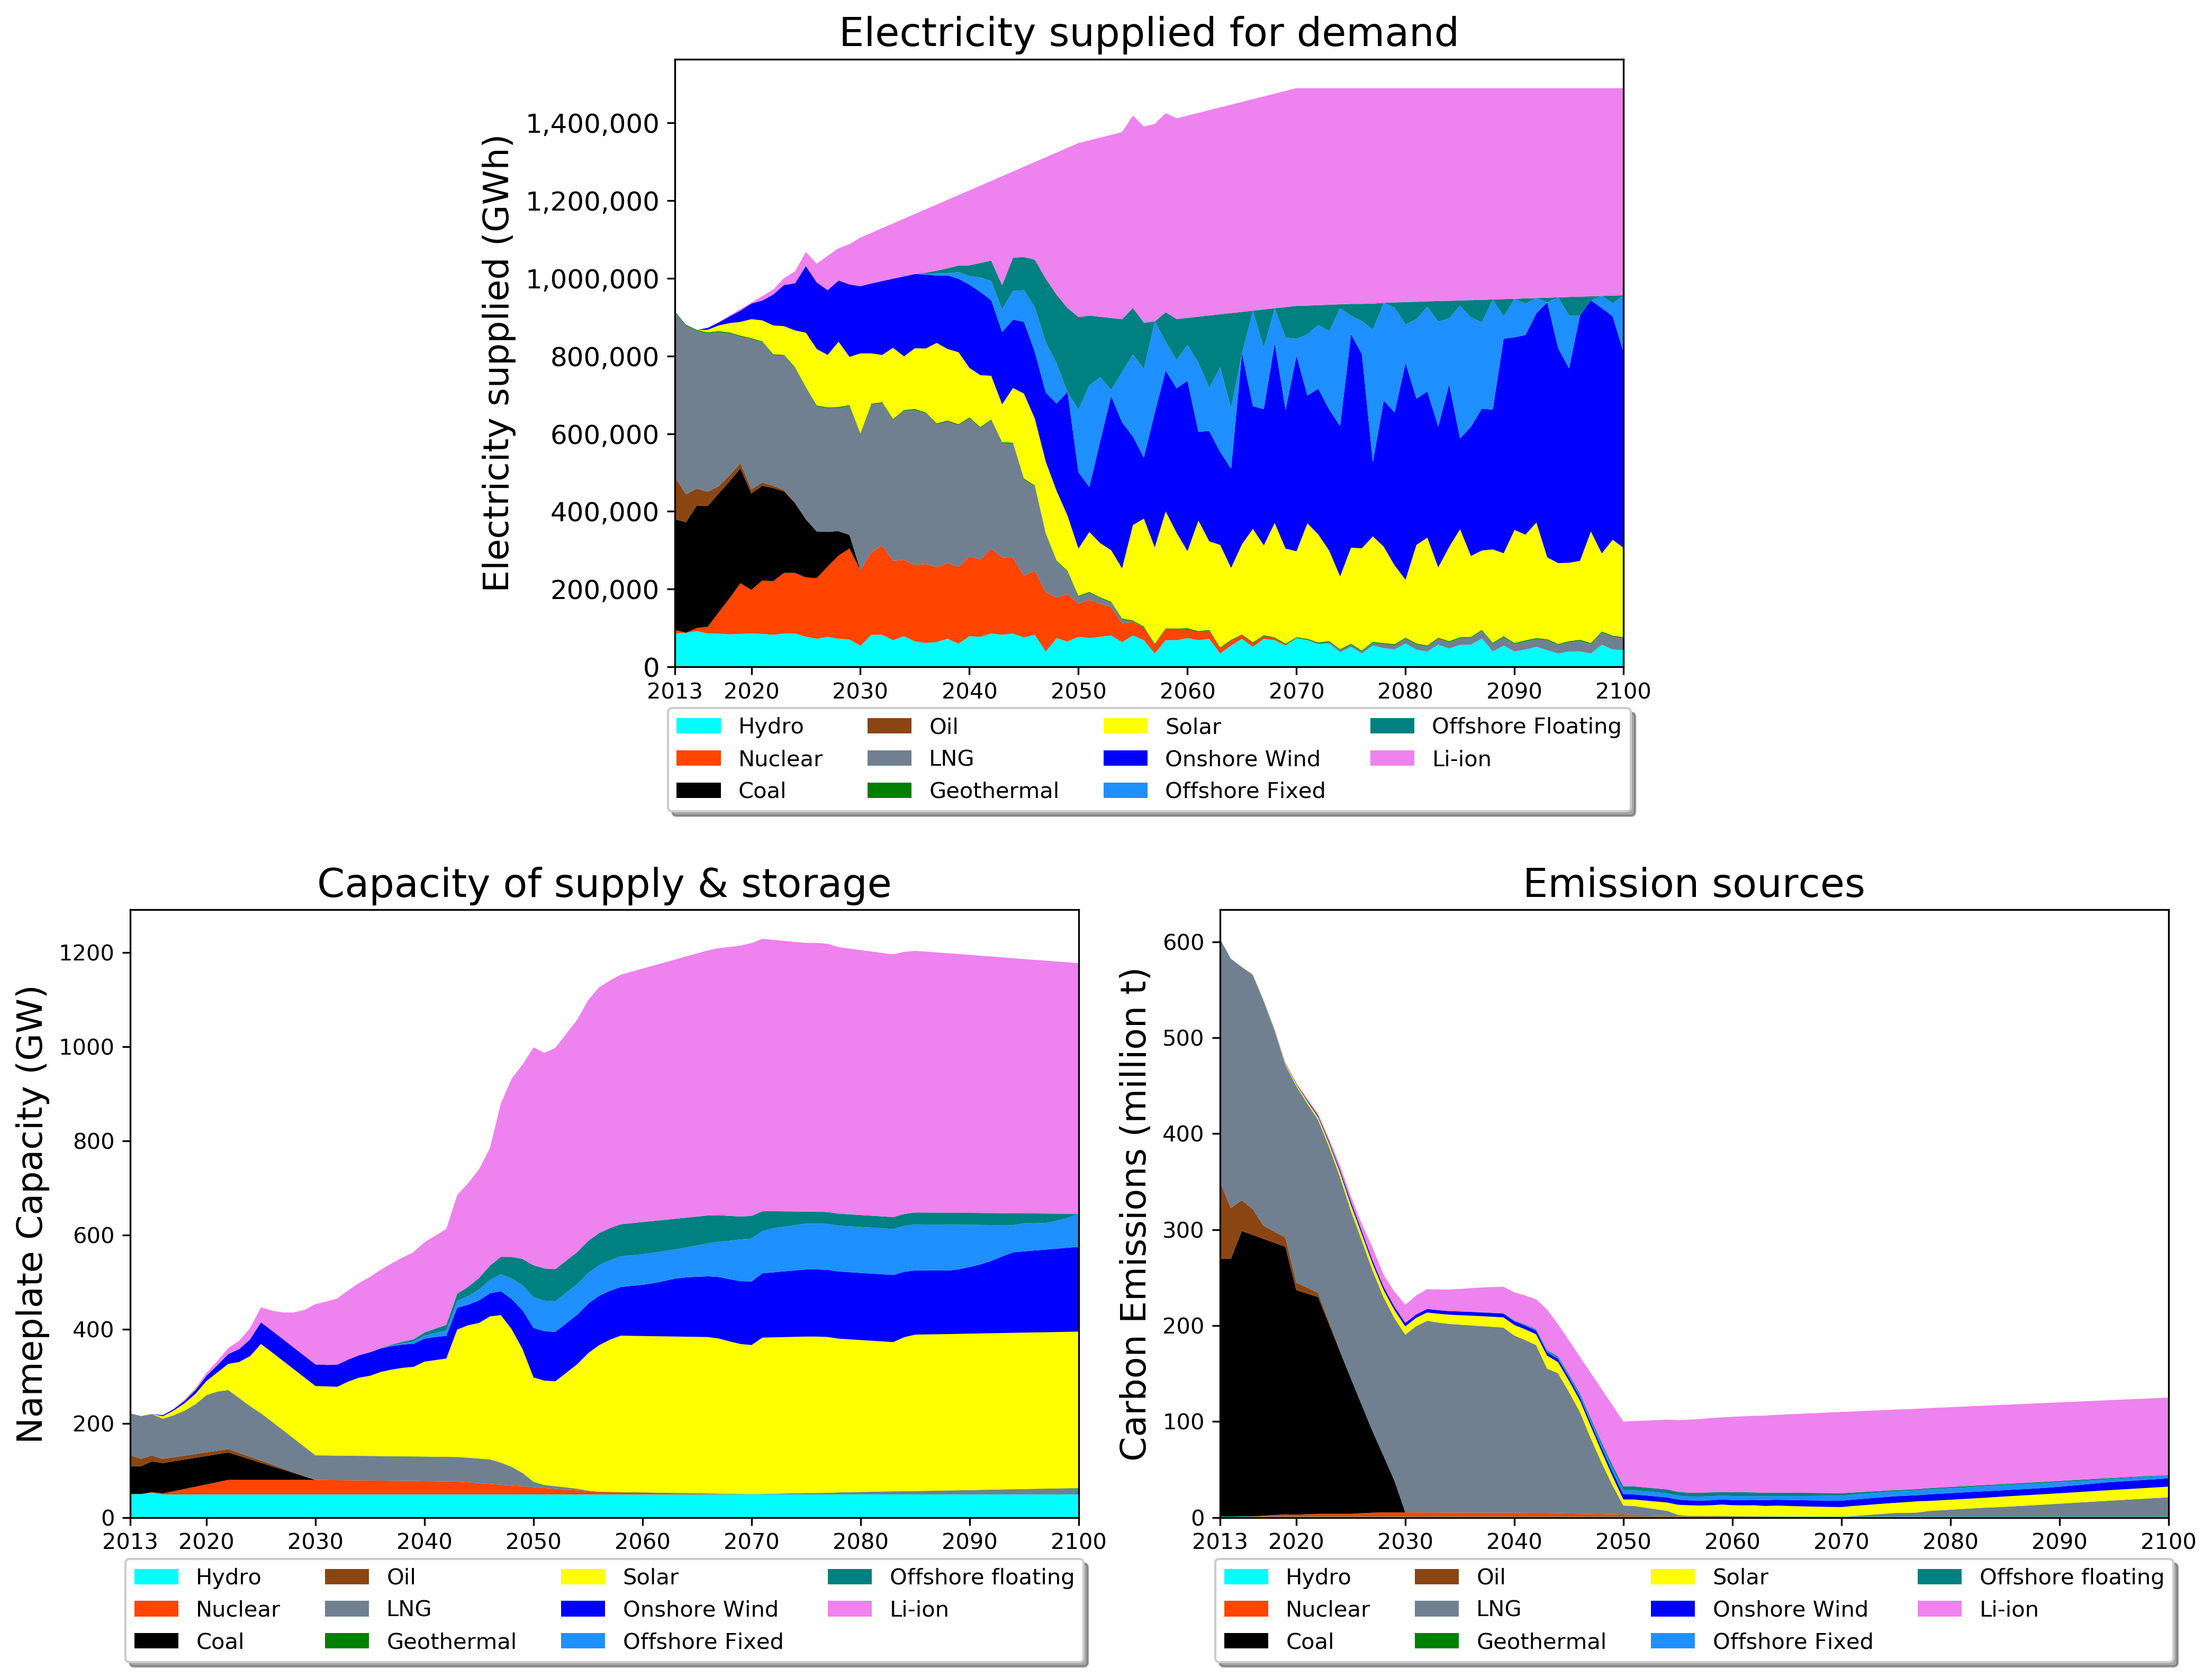
\includegraphics[scale=0.25]{figures/conv_nonuc}
\caption{Conventional technologies, no new nuclear.}
\end{figure}

\begin{figure}[h] 
\centering
\label{scen2}
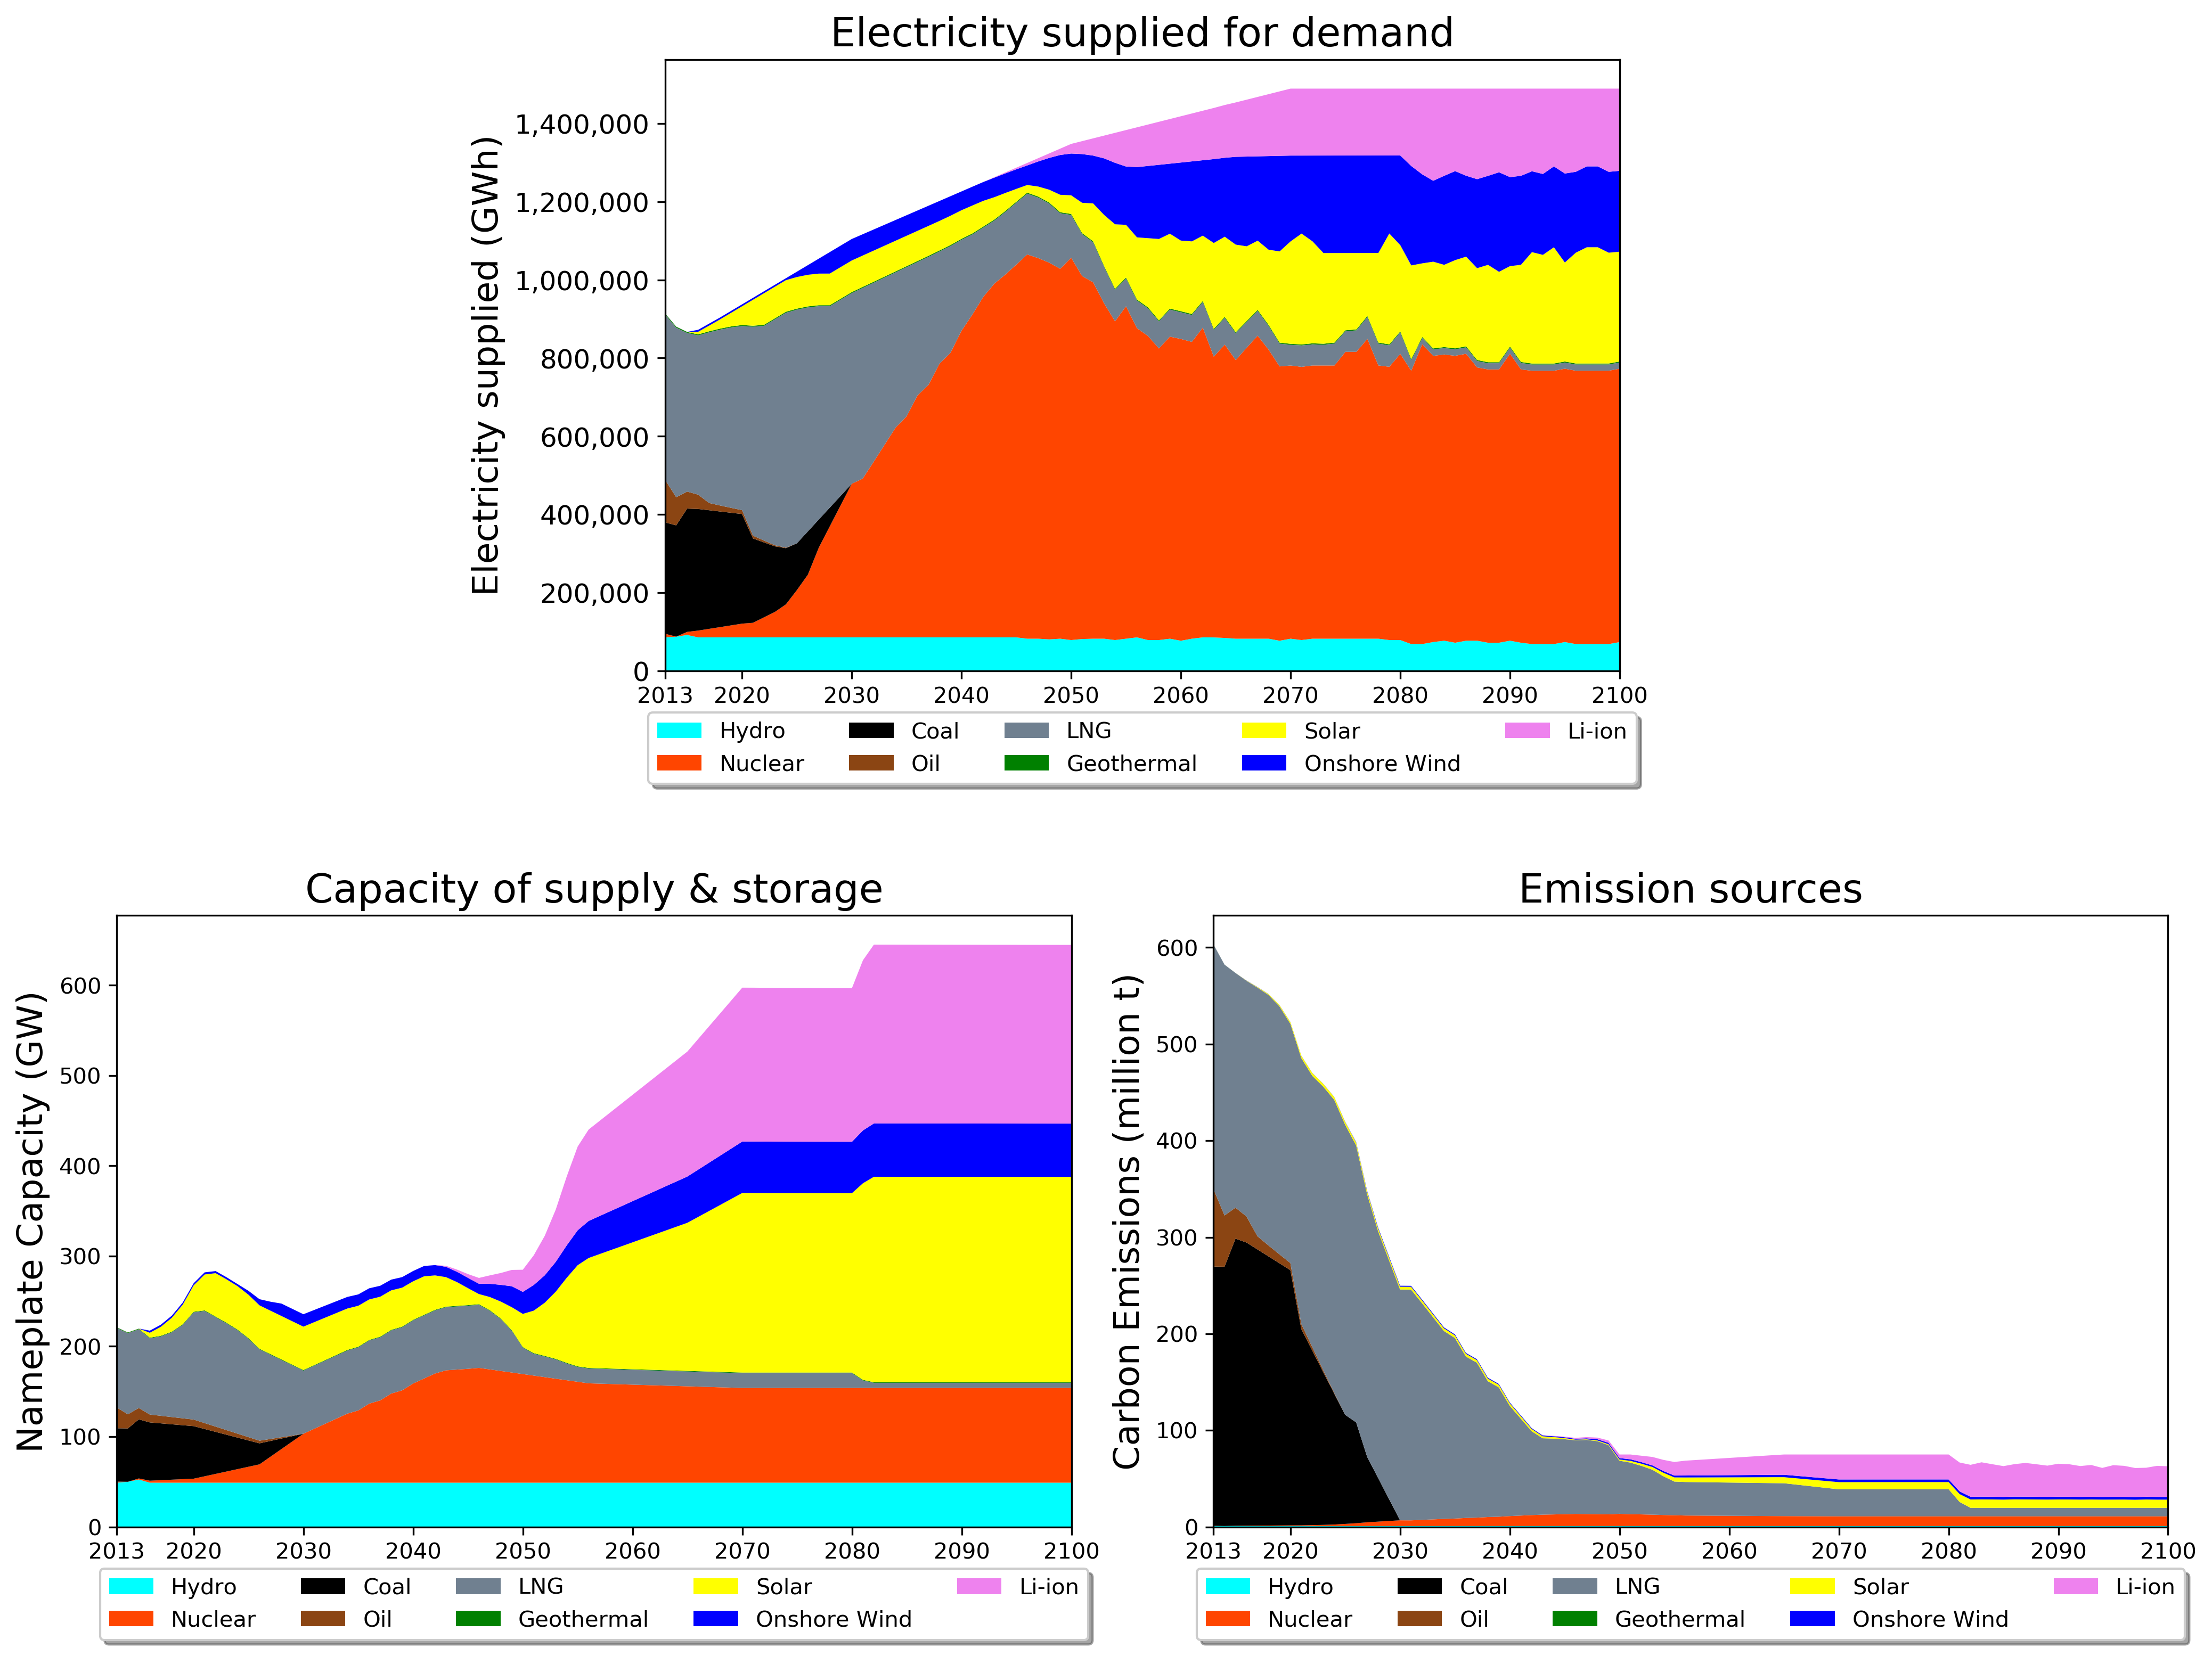
\includegraphics[scale=0.25]{figures/conv_nuc}
\caption{Conventional technologies, with new nuclear.}
\end{figure}

\begin{figure}[h] 
\centering
\label{scen3}
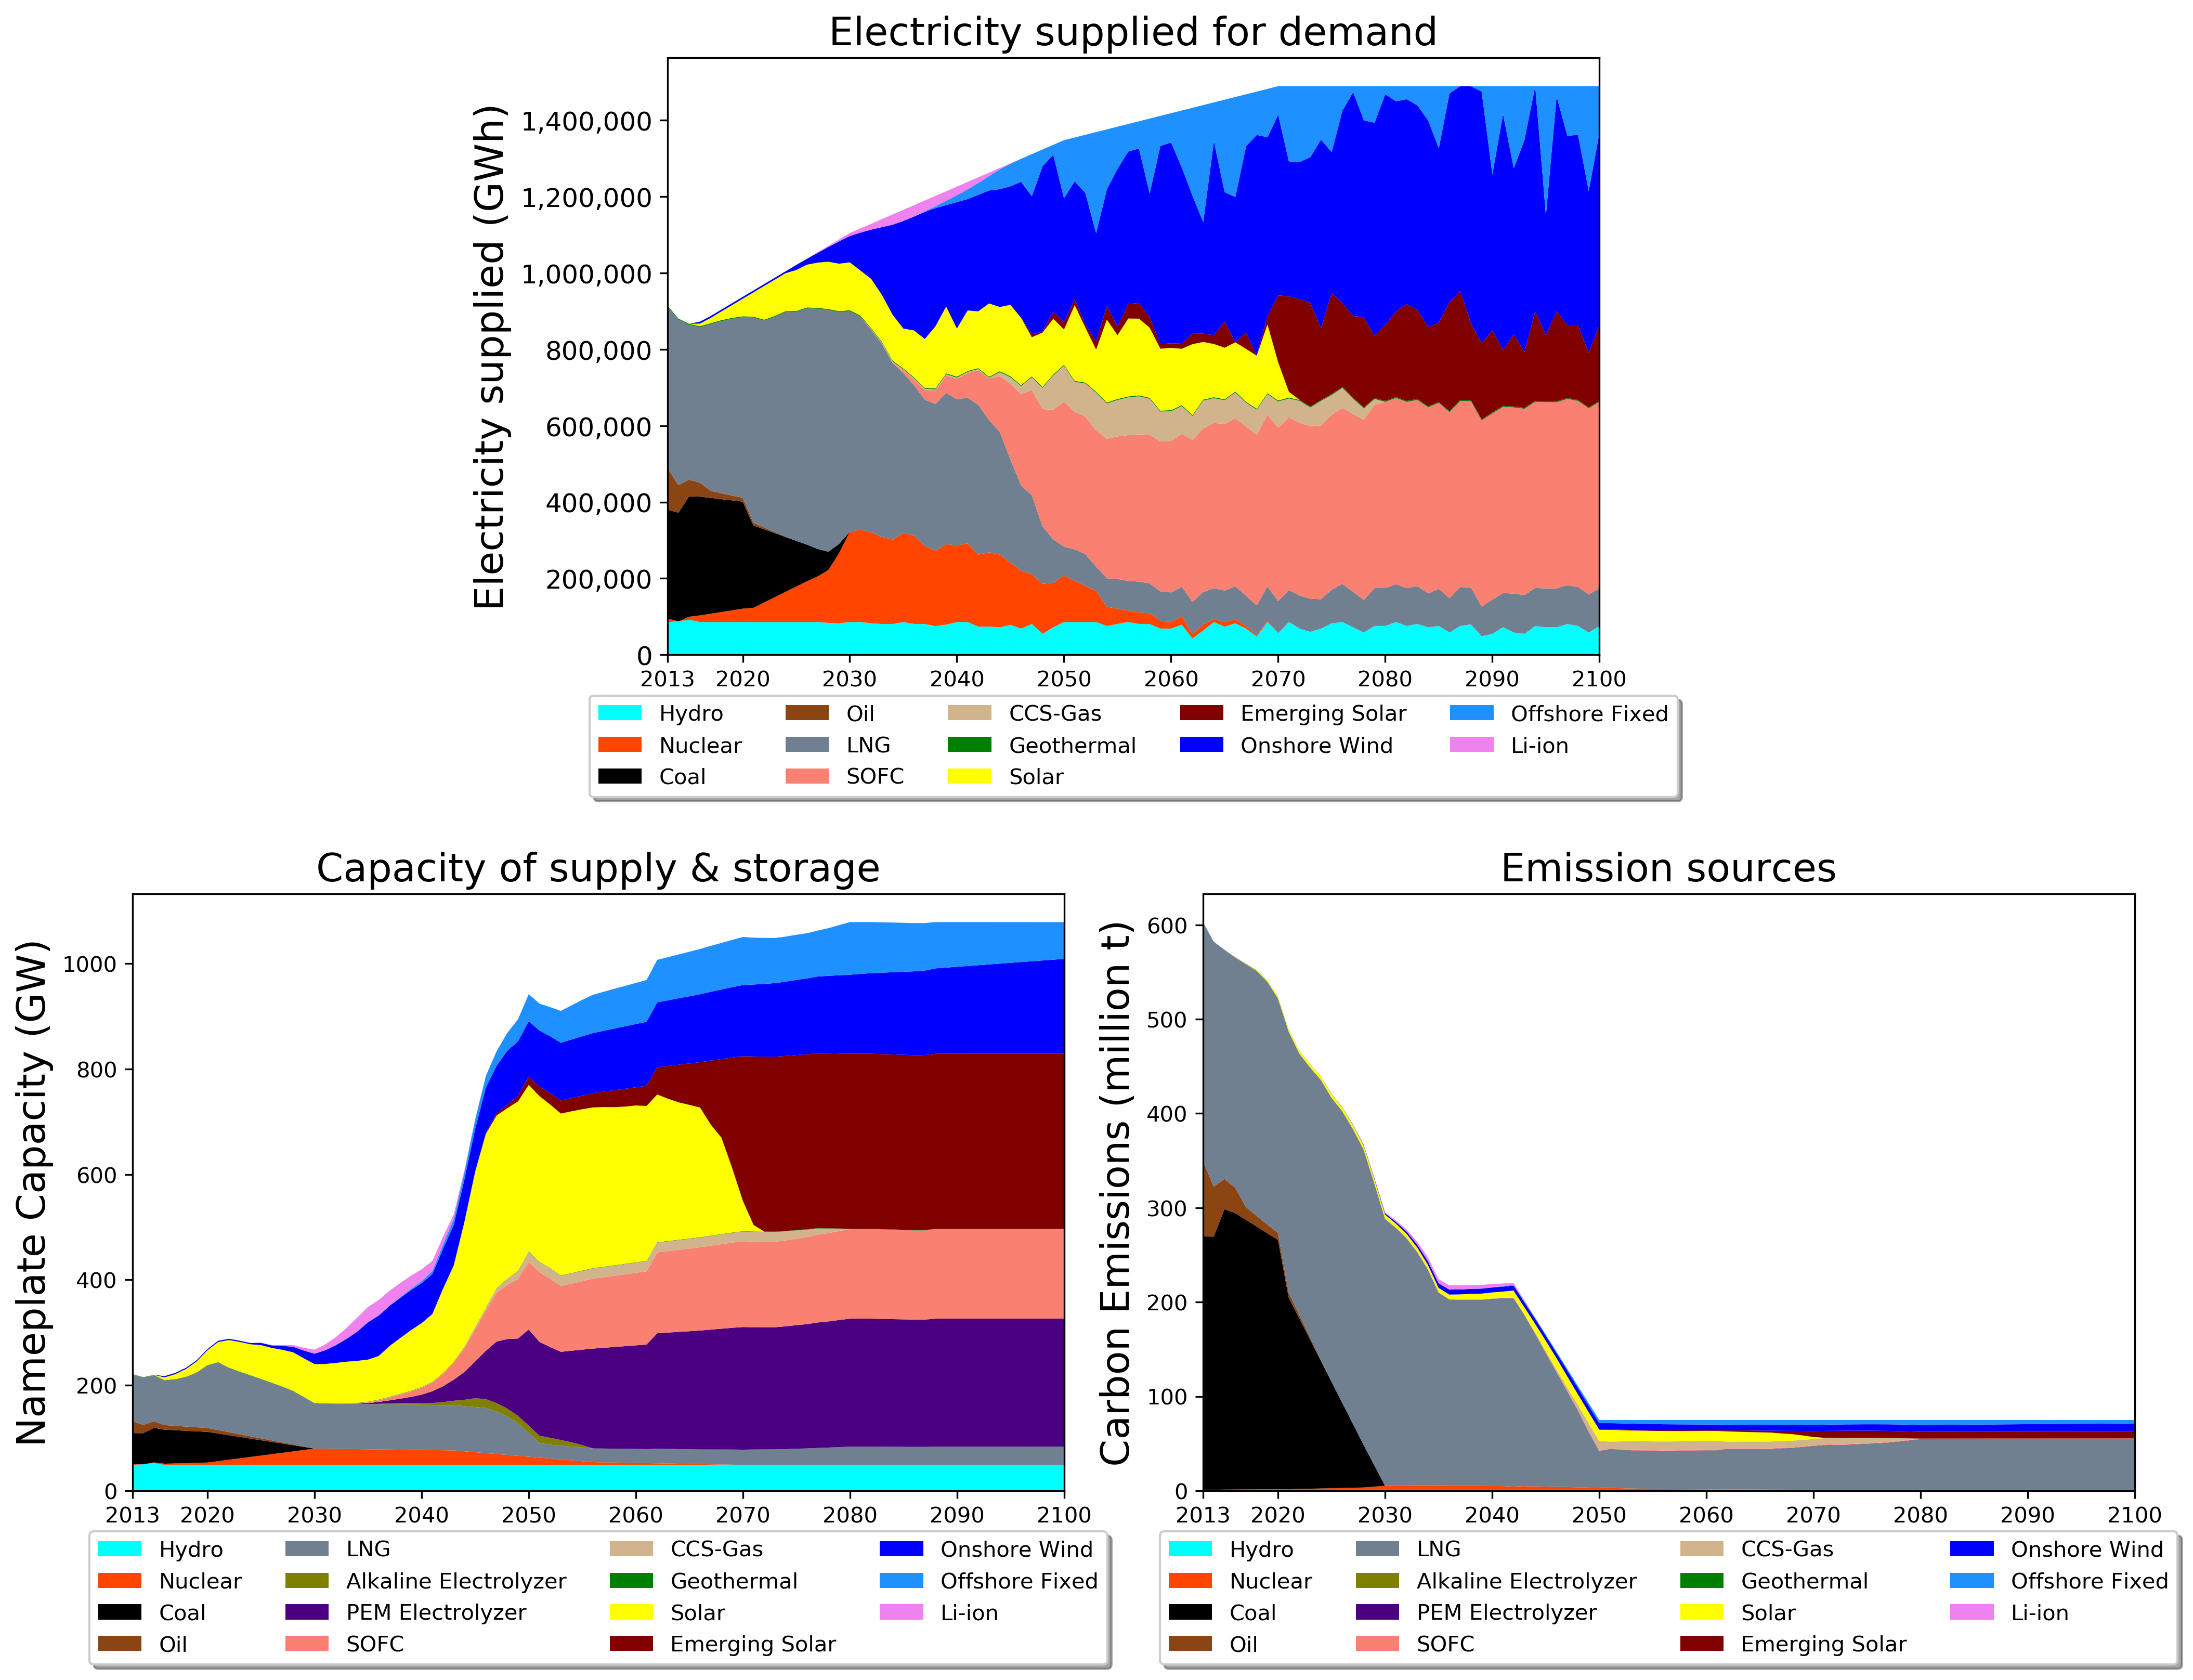
\includegraphics[scale=0.2]{figures/newtechs_nonuc}
\caption{Emerging technologies, no new nuclear.}
\end{figure}

\begin{figure}[h] 
\centering
\label{scen4}
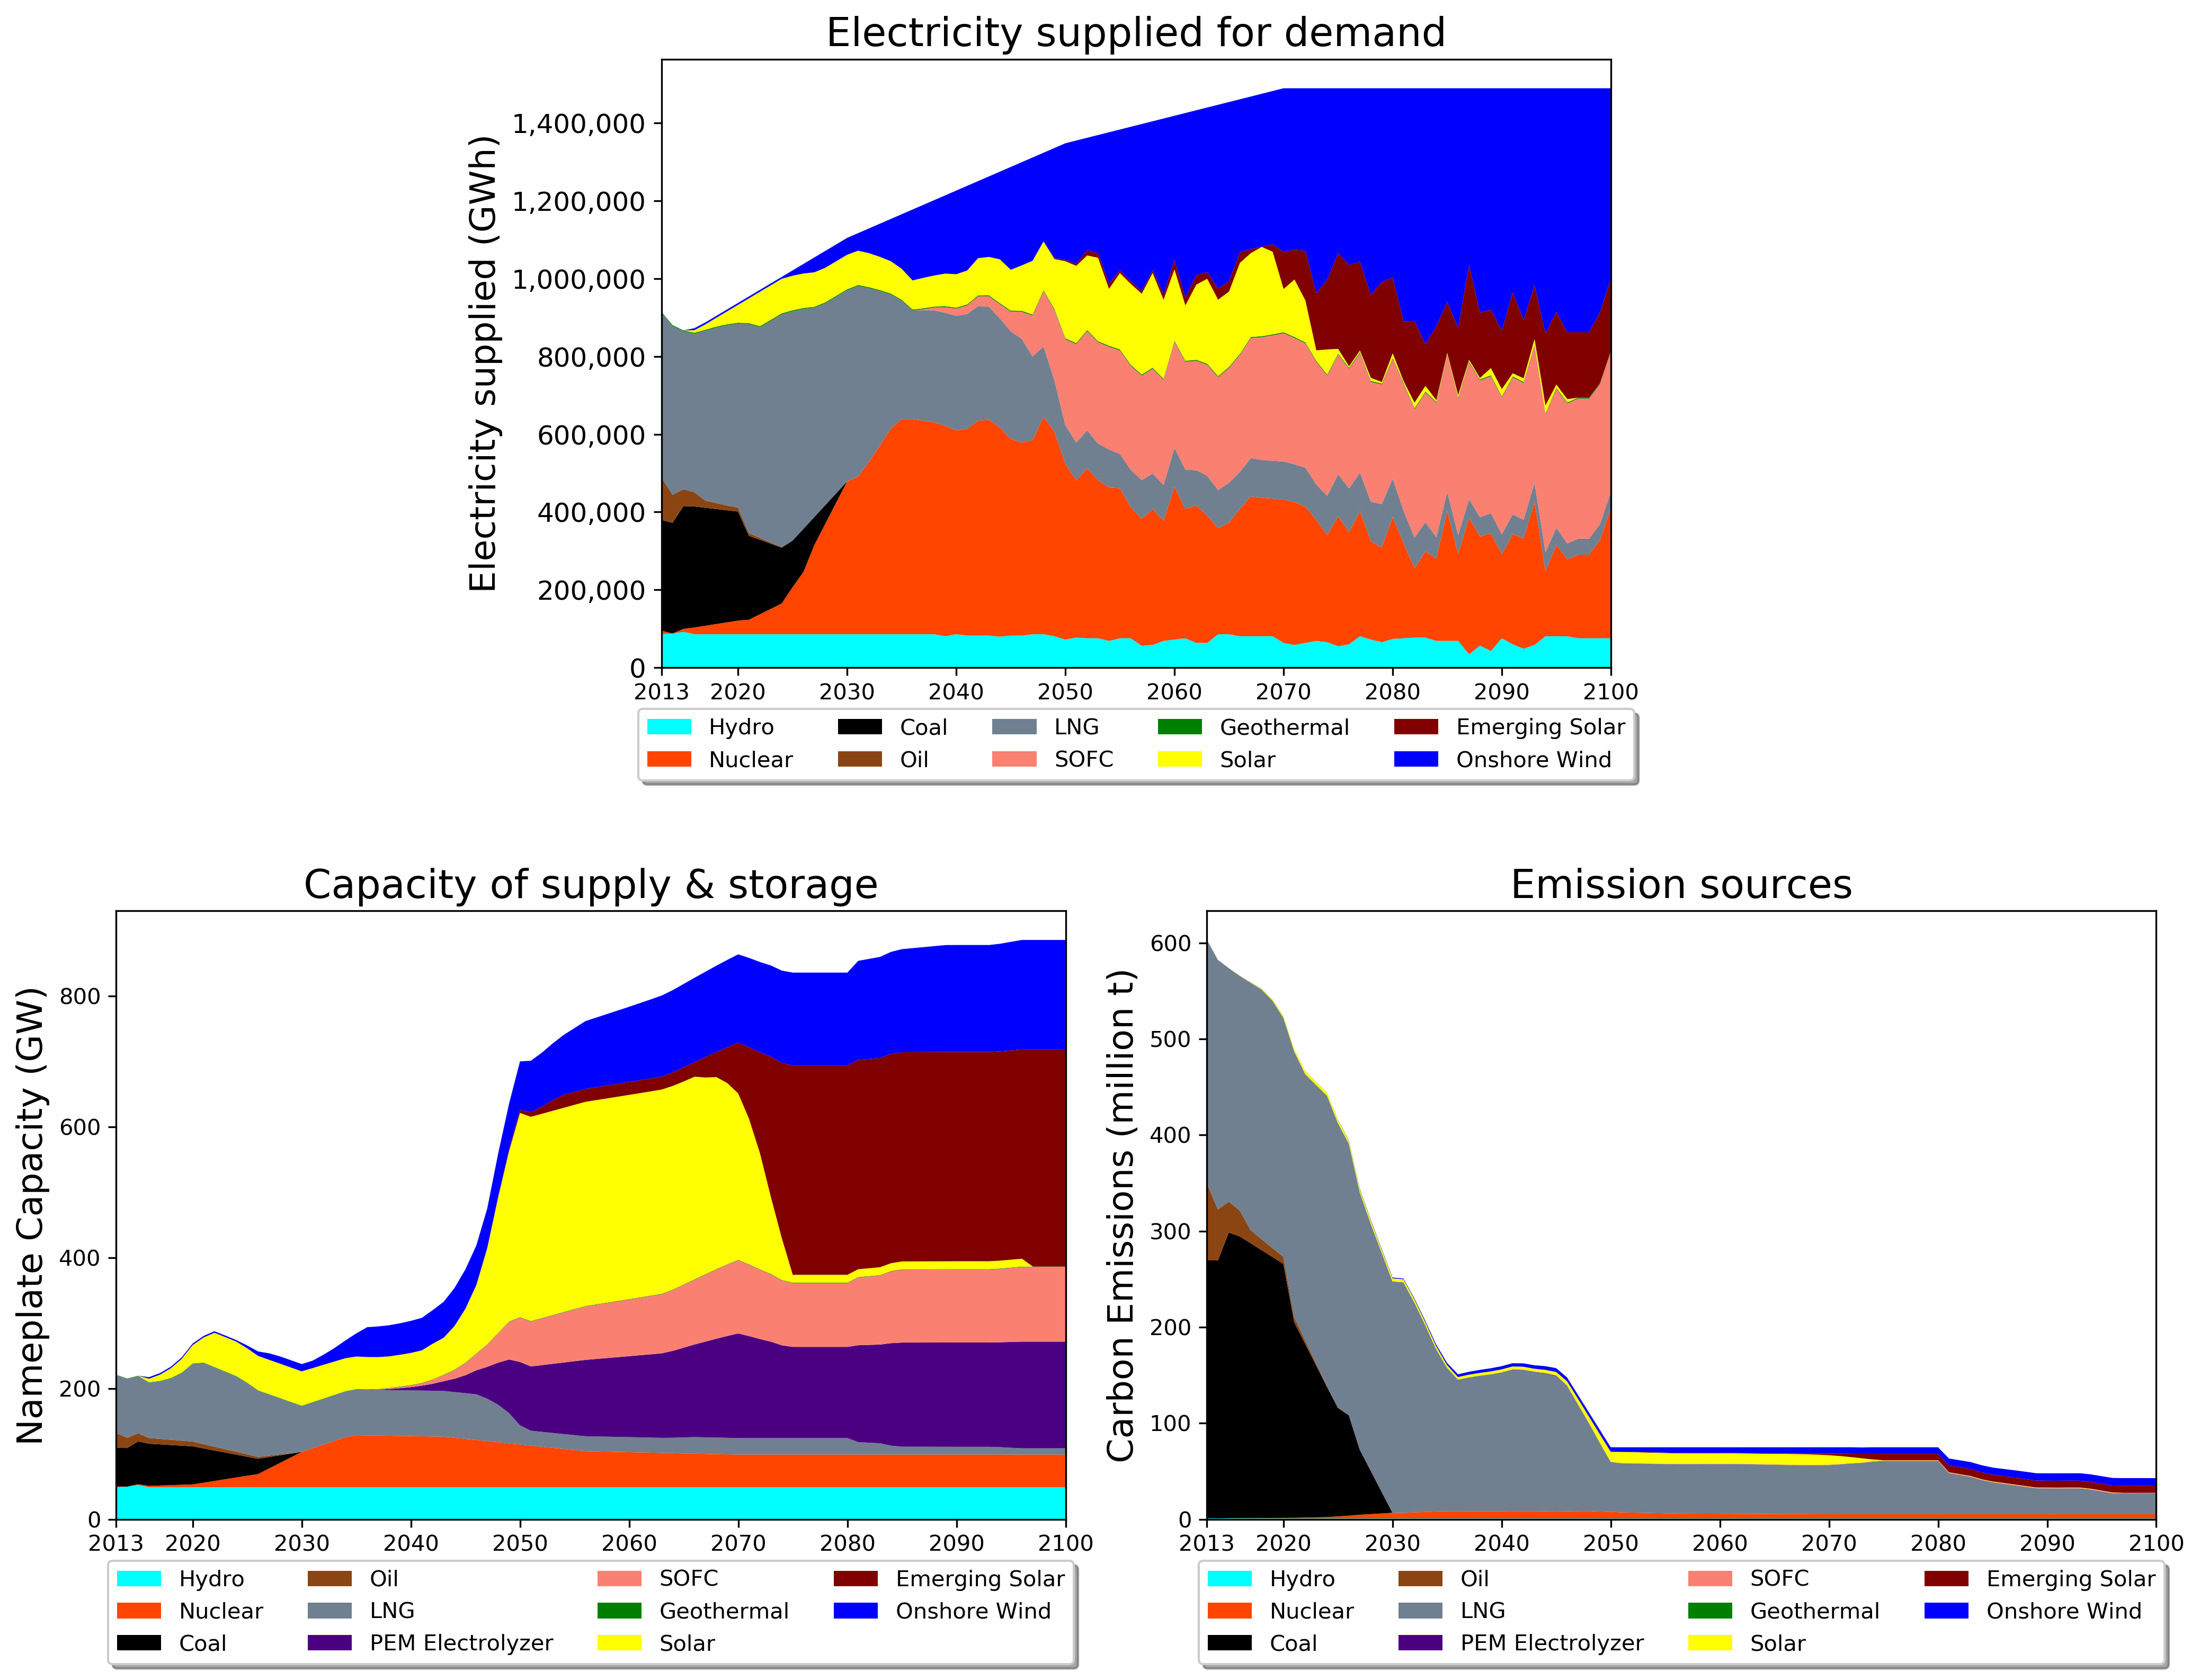
\includegraphics[scale=0.2]{figures/newtechs_nuc}
\caption{Emerging technologies, no new nuclear.}
\end{figure}


\FloatBarrier
\section{Discussion}
% This should explore the significance of the results of the work, not repeat
% them. A combined Results and Discussion section is often appropriate. Avoid
% extensive citations and discussion of published literature.

%Notes for Ansh:
%Importance of nuclear : cost of various transitions, flexibility by itself and when coupled with storage (Li-ion, H2). How it precludes the need for CCS.
%Urgency of transition : scenarios + sensitivity analysis.
%Li-ion storage: land use requirements for each case, qualitatively discuss Co, Ni requirements. Say Li is okay.
%AECs,PEMECs,SOECs need to be highly flexible with high availability factors.
%SOFCs: need for extremely responsive SOFCs with high availability factor, flexible operation (cite challenges from NREL).
%pemecs still part of cost optimal solutions
%identify key techs, same fcs needed always
%nuclear is key
%pws will have to be cheaper/cost competitive with electrolyzers to have a role
%main H2, role of CCS LNG - secondary alternative to H2 - as shown by correlation with SOFC inv cost. Not good on its own. Supplement to H2.
%H2 non trivial despite large range of perturbation
% FC flexibility, more storage/H2 less flex for CCS, nuclear

%urgency
As the results of all base case scenarios indicate, rapid retirement of fossil fuels and deployment of carbon neutral technologies is urgently required to achieve emission reduction targets in Japan. All coal and oil plants need to be shut down between 2025-2030, and natural gas use must be reduced dramatically. It is also imperative that the existing nuclear reactors be operated at full capacity by 2022. Since hydrogen plays a key role in zero to moderate nuclear deployment scenarios (Figs. \ref{scen3} and \ref{scen4}), it appears prudent to invest in hydrogen power. As the model uses learning curves for technology prices and our objective function is transition cost, hydrogen technologies are deployed as late as possible in order to minimize costs by utilizing technologies at their cheapest, while there is still time to deploy them and achieve emission goals. Therefore,  results indicate that it is imperative that Japan deploy an increasing amount of renewables including wind power between 2020-2030, and be prepared to deploy and rapidly scale up hydrogen power by 2030 at the latest in the absence of new nuclear, or by 2035 with new nuclear.

%nuclear
The scenario with the largest nuclear deployment, Scenario 2, also has the lowest transition cost. When used with hydrogen, 50 MW of new nuclear results in the greatest reduction in emissions after 2050 out of all 5 scenarios. It also reduces the cost of the transition from 3.18 Trillion USD in Scenario 3 to 2.80 Trillion USD in Scenario 4, a difference of 12\% of the system cost. The estimated savings in cost and emissions due to nuclear are conservative, as we have not incorporated the cost of transporting hydrogen utilizing tankers or pipelines. The large emission cuts achieved with the help of nuclear also allow natural gas to continue operating until 2100, while meeting emission goals. As natural gas is well suited to peaking and load-following, when coupled with flexible fuel cell technologies, it could engender in an extremely stable energy system. 

For the transitioning energy system in Japan, under all scenarios investigated, nuclear plays a key role in reducing emissions. A potential strategy for Japan could include the reinvigoration of its nuclear energy sector by restarting existing plants, and if politically feasible, constructing new plants, and investing in advanced reactor research. To minimize the environmental impact from life cycle emissions, it is necessary that all existing and any new reactors be operated for a lifetime of 60 years or more at a high capacity factor. Premature decommissioning due to operational problems or lack of public acceptance need to be avoided. Therefore, prioritizing reactor safety for resilience to disasters and in order to regain the public's trust in nuclear power, and increasing public awareness of nuclear's vital role in mitigating carbon emission is key to achieving 2030 and 2050 emission targets.

%renewables and flexibility
In all scenarios, solar and wind supply a large portion of the electricity demand. Unless large numbers of nuclear power plants are constructed, Japan will need to invest heavily in offshore wind farms by 2030 (Figs. \ref{scen1},\ref{scen3}-\ref{scen5}). If hydrogen and CCS are not deployed by 2035, investment in offshore floating turbines may also become necessary (Fig. \ref{scen1}). Under a scenario with a relatively large share of renewables, grid flexibility becomes extremely important. Such a scenario requires significant investment in storage technologies, and ensuring that all emerging technologies are flexible and responsive. As natural gas is the only extant option for load-following, it is necessary to invest in nuclear or hydrogen to achieve emission cuts while simultaneously keeping natural gas operational for load-following. Additionally, any nuclear power plants and fossil fuel power plants which use CCS must be able to load-follow, or be coupled to storage, ideally electrolysers, in order to store excess electricity for peak demand. Any fuel cell technology utilized must also be extremely flexible and responsive. Since the model prioritizes \gls{SOFC}s over \gls{PEMFC}s due to their higher efficiency, it is important that \gls{SOFC}s reduce their startup times to have an edge over \gls{PEMFC}s in utility-scale applications.

%batteries
Lithium-ion is the preferred storage medium in the absence of hydrogen. However, as the base case scenarios indicate, extremely large capacities of storage must be deployed to achieve a stable grid that can sustain the large capacities of renewables required for deep emission cuts. While lithium may be available, cobalt and manganese reserves are limited \cite{scrosati_lithium-ion_2011,simon_potential_2015,turcheniuk_ten_2018} , which may inflate the prices of lithium-ion storage if it is relied upon as the primary storage medium. It may be preferable to redesign batteries to reduce the amount of rare minerals used in their manufacturing, and improve recycling to increase the recovery rate of rare metals. The life cycle emissions from batteries must also be reduced by using cleaner materials and electricity for manufacturing. If hydrogen storage is available, battery storage storage serves as a near-term transition technology after which hydrogen storage dominates (Figs. \ref{scen3}-\ref{scen5}).

%hydrogen - key players, key parameters, path forward?
After nuclear, hydrogen power emerges as the second most efficacious technology for achieving 2050 emission goals. As seen in the sensitivity analysis results, hydrogen maintains a significant share of the electricity mix despite a wide range of perturbations to key parameters of the hydrogen sector. While \gls{SOFC}s and \gls{SOEC}s are preferred over \gls{PEMFC}s and \gls{PEMEC}s in all of our simulations, the role of hydrogen is so important that if \gls{SOFC} or \gls{SOEC} deployment is disabled, the model replaces them with inferior \gls{PEMFC}s or \gls{PEMEC}s respectively to recreate similar energy mixes. Key technologies that aid in decarbonization in our simulations are \gls{SOFC}s and \gls{PEMEC}s, which are close to maturation. Steam reforming, with or without CCS, does not get utilized in our simulations due to its high emission coefficient. At the lower end of the technology readiness scale, \gls{SOEC}s emerge as tremendously disruptive due to their high efficiency. However, their operational lifetimes need to be increased significantly, life cycle emissions must be kept low, and cost-competitiveness with \gls{PEMEC}s must be achieved in order to realize their potential. \gls{PWS} plays a marginal role as it is not cost-competitive with electrolysis. From the simulation output data, the investment cost of \gls{SOFC}s emerges as a critical parameter. Therefore it is vital to reduce fuel cell investment costs to make deep emission reduction economically feasible. However, low response times and high availability are two other key factors that are implicit in our assumptions. If \gls{SOFC}s are not as flexible as assumed, they are replaced in our simulations by \gls{PEMFC}s, which are known to be more flexible and closer to commercialization. In Scenarios 3 and 4, solar, wind, and nuclear are used to generate hydrogen. Therefore it would be economically favourable to couple utility-scale renewables and nuclear power plants with electrolysis plants. Waste heat from nuclear could also be used to produce hydrogen, and would reduce reliance on renewables for electrolysis. As mentioned previously, more flexible and responsive fuel cells and electrolyzers are likely to be the dominant technology in such a system.

%ccs
CCS plays a small role in our base case scenarios as a transitional technology, despite being cheaper than hydrogen. Its share is found to be largely insensitive to its investment costs as evidenced by the sensitivity analysis. This is mainly due to its large emission coefficient. Marginal gains are expected in its penetration if the efficiency of CCS is increased to reduce its direct emissions. Reducing indirect emissions is likely to have a greater impact. This could be achieved in the future by increased electrification of the industrial sector, and the use of hydrogen to produce steel.

Although our analysis relies on optimal solutions and scenarios and is technologically agnostic, policy makers in Japan will face difficult future decisions as to the long-term nature of the low-carbon energy system. One approach could be to prioritize nuclear energy and to reap the benefits of inexpensive, low-carbon energy, at the cost of achieving consensus from the public for its long-term deployment and use. Another low carbon energy pathway proposed by our results is a transition toward a hydrogen economy, utilizing hydrogen as a storage medium to engender significant deployment of renewable energy. The hydrogen pathway also provides more energy security, obviating the use of coal and oil and mitigating the use of natural gas. As social opposition to nuclear is a prominent issue in Japan, the deployment of a parallel nuclear and hydrogen-based energy system is unlikely. However, our results indicate that these two approaches are not mutually exclusive. The cost of transitioning to a hydrogen energy system without deploying any new nuclear is much higher than that of any of the nuclear-inclusive options. Deploying nuclear in tandem with hydrogen provides a cost-effective compromise. An approach reliant on a mature technology like nuclear also improves the likelihood of Japan meeting its 2050 emission goals, as at the time of writing, the timely success of the Japanese hydrogen plan is far from certain. At the very least, as is the case for CCS and fossil fuels, nuclear power may offer a "bridging" option, providing a low-carbon pathway in the short term through extended nuclear lifetimes and limited new builds, allowing sufficient time for the maturation of hydrogen and renewable-based energy options for longer-term deployment timelines. If supported politically, long-term use of nuclear power could provide emission cuts well beyond the 2050 targets. Policy which is cognizant of these economic, environmental, and social aspects of energy systems is required to deliver a low-cost, low-carbon energy future for Japan which is socially acceptable.
\FloatBarrier
\begin{frame}
  \frametitle{Conclusion}
        We showed many things.
        \begin{itemize}
                \item Cats are peculiar
                \item Blue and Orange are fierce colors
                \item Math can be rendered nicely
                \item Cite your sources
        \end{itemize}
\end{frame}

\FloatBarrier
\section{Acknowledgments}

The author(s) gratefully acknowledge the support of the International Institute for Carbon Neutral Energy Research (WPI-I2CNER), sponsored by the Japanese Ministry of Education, Culture, Sports, Science and Technology. We are also grateful to Kenshi Itaoka and Hadi Farabi-Asl for providing valuable discussions related to this project, and to Gavin Davis and Nataly Panczyk for editing drafts.

The authors contributed to this work as described below.

Anshuman Chaube designed simulation models, conducted sensitivity analysis, and wrote the original draft of the paper.

Andrew Chapman conceived and contributed to conception of the simulations, designed simulation models, and wrote the original draft of the paper. 

Akari Minami translated data from Japanese to English, and assisted with testing and performing simulations.

James Stubbins supervised the work, conceived and contributed to conception of the simulations, and reviewed drafts of the paper.

Kathryn D. Huff supervised the work, conceived and contributed to conception of the simulations, and reviewed drafts of the paper.  Prof. Huff is supported by the Nuclear Regulatory Commission Faculty Development Program, the National Center for Supercomputing Applications, the International Institute for Carbon Neutral Energy Research (WPI-I2CNER), sponsored by the Japanese Ministry of Education, Culture, Sports, Science and Technology, and  DOE ARPA-E MEITNER program award DE-AR0000983.

\FloatBarrier
\bibliographystyle{elsarticle-num}
\bibliography{i2cner-paper-2}
\newpage
\appendix
\section{Data and assumptions for scenarios} \label{Appendix}

\begin{table}[!ht]
	\caption{Data for initial condition.}
	\vspace{0.1in}
	\begin{tabularx}{1.2\textwidth}{p{0.35\textwidth} p{0.25\textwidth} p{0.2\textwidth} p{0.25\textwidth}}
		\hline
\textbf{Technology} & \textbf{\gls{lcoe}} \cite{lazard_lazards_2016} & \textbf{Emission} & \textbf{Year of total}\\
  & (USD/kWh) & \textbf{Coefficients} \cite{noauthor_electricity_2019} (gCO$_2$-eq. /kWh) & \textbf{retirement} \\
\hline
Coal & 0.06 & 943 & 2030 \\
\gls{lng} & 0.08 & 599 & 2030 \\
Oil & 0.39 & 738 & 2030 \\
Nuclear & 0.11 & 21 & 2069 \\
Hydro & 0.05 & 11 & N.A. \\
Geothermal & 0.12 & 13 & N.A. \\
Wind & 0.11 & 25 & 2040 \\
Solar & 0.15 & 37 & 2040 \\
\hline 
\end{tabularx}
\label{init-eco}
\end{table}

\begin{figure}[h] 
\centering
\label{ic-elc}
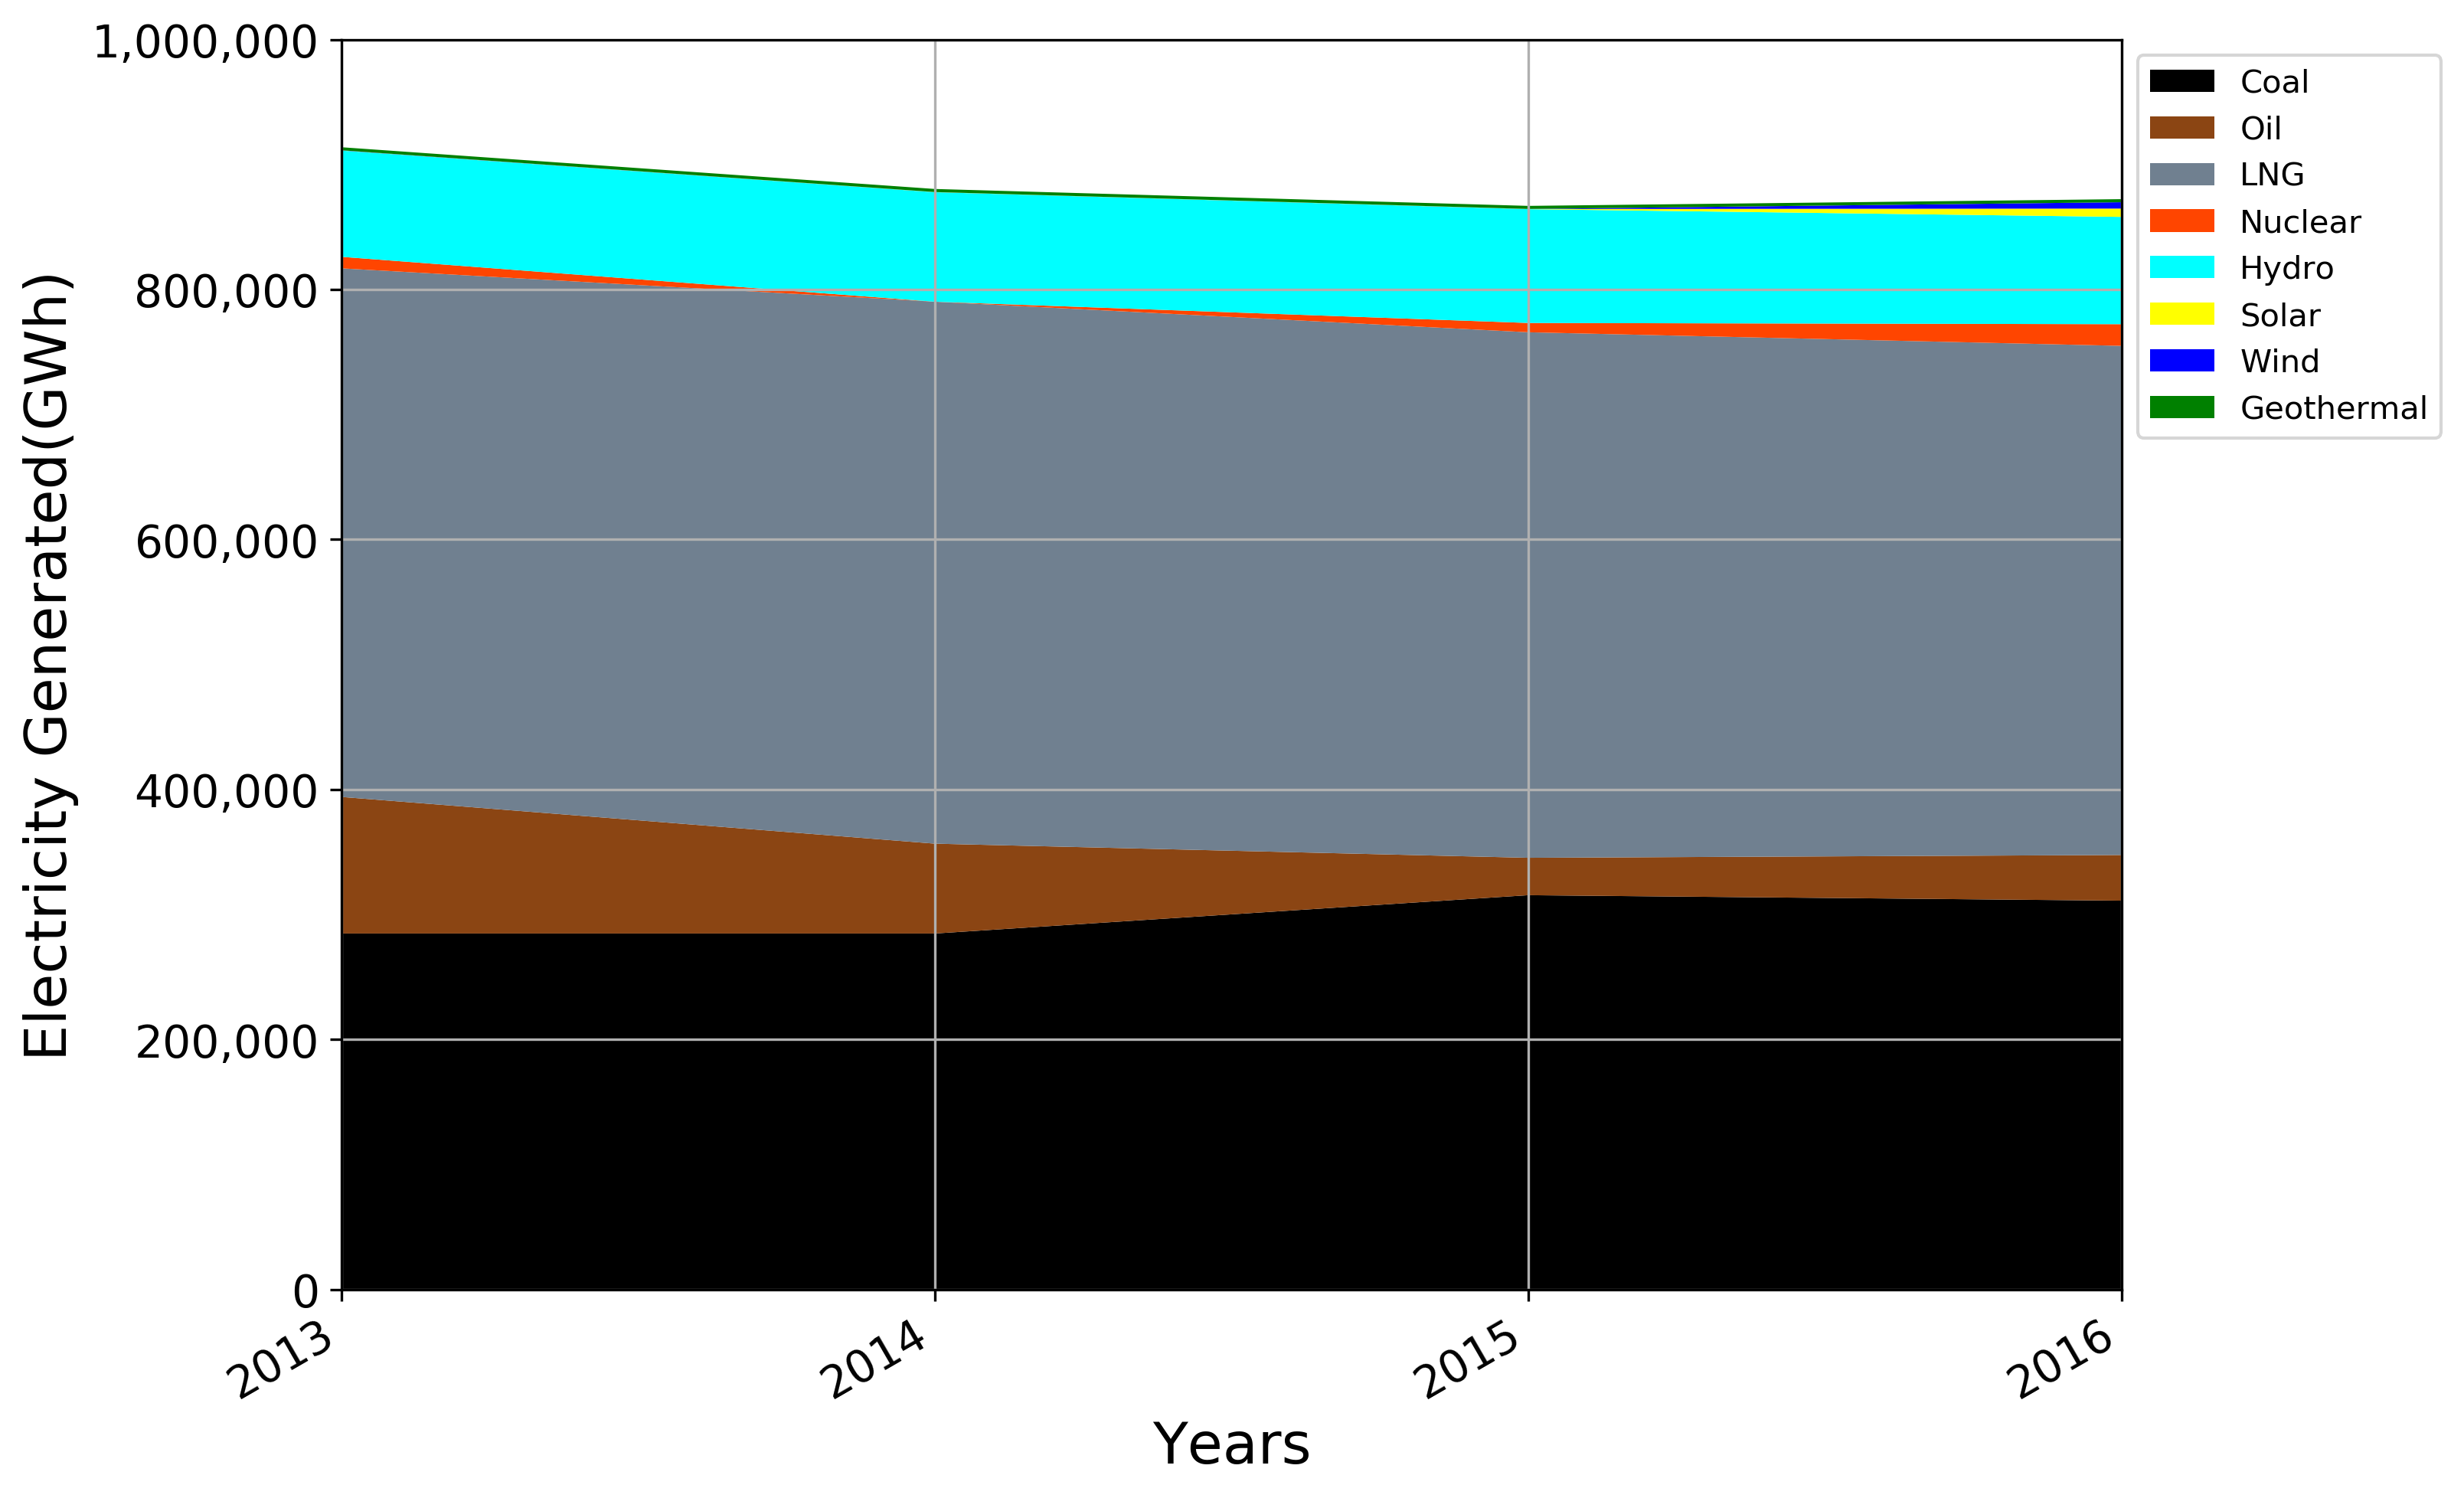
\includegraphics[scale=0.5]{figures/IC}
\caption{Electricity generation that defines the initial condition of the model.}
\end{figure}

\begin{table}[!ht]
	\caption{Initial condition CO$_2$ emissions compared to the model and data from the Carbon Trust\cite{carbon_brief_carbon_2018}.}
	\vspace{0.1in}
	\begin{tabularx}{\textwidth}{p{0.08\textwidth} p{0.35\textwidth} p{0.35\textwidth} p{0.15\textwidth}}
		\hline
\textbf{Year} & \textbf{Model Emissions} & \textbf{Actual Emissions} & \textbf{Error} \\
  & Mt CO$_2$-eq. & Mt CO$_2$-eq. &  \\
\hline
2013 & 603.62 & 592.4 & 1.89 \% \\
2014 & 582.27 & 572.6 & 1.69 \% \\
2015 & 572.53 & 560.3 & 2.18 \% \\
2016 & 565.94 & 552.8 & 2.38 \% \\
\hline 
	\end{tabularx}
\label{ic-co2}
\end{table}

\begin{landscape}
\begin{longtable}{ |*{8}{c|} }
\caption{Economic data for modelled technologies.}\\
\hline
\textbf{Technology} & \textbf{Capital} & \textbf{Fixed} & \textbf{Variable} & \textbf{Lifespan} & \textbf{Capacity Factor/} & \textbf{Emission} & \textbf{Year} \\
 & \textbf{Cost} & \textbf{\gls{OM}} & \textbf{\gls{OM}} &  & \textbf{Efficiency} & \textbf{Coefficient} & \textbf{available} \\
 & MUSD/GW & MUSD/GW & MUSD/GWh & Years  &  & gCO$_2$/kWh  &  \\
\hline
\endhead  % header material
\hline
\endfoot  % footer material
\hline
\endlastfoot
\gls{USC} \cite{eia_cost_2020,ipcc_2014} & 3661 & 40.41 & 0.045 & 40 & CF=0.55 & 820 & 2017 \\
\gls{lng}\cite{eia_cost_2020,ipcc_2014} & 1079 & 14 & 0.0025 & 30 & CF=0.55 & 490 & 2017 \\
Nuclear \cite{eia_cost_2020,ipcc_2014,lokhov_load-following_2011} & 6317 & 121.13 & 2.36 & 60 & CF=0.6-0.95 & 12 & 2017 \\
Li-ion Storage \cite{mongird_energy_2019,emilsson_lithium-ion_2019} & 1876 (2017) & 10 & 0.3 & 10 & Eff=0.86 & 151(2017) & 2017 \\
 & 1446 (2025) &  &  &  &  & 87(2050) &  \\
Solar \cite{eia_cost_2020,ipcc_2014} & 1307(2017) & 15.19 & 0  & 25 & CF=0.14 & 37 & 2017 \\
 & 615(2050) & & & & & &  \\
Onshore Wind & 3454(2017) & 136.37 & 0 & 25 & CF=0.25(2017) & 20(2017) & 2017 \\
\cite{eia_cost_2020,ipcc_2014,kato_energy_2016,govindji_appraisal_2012,heger_wind_2016} & 2406(2050) &  &  &  & CF=0.35(2050) & 7 (2040) &  \\
Offshore Wind(Fixed) & 7772(2017) & 341 & 0 & 25 & CF=0.3(2017) & 25(2017) & 2017 \\
\cite{eia_cost_2020,ipcc_2014,kato_energy_2016,govindji_appraisal_2012,heger_wind_2016} & 3381(2050) &  &  & & CF=0.40(2050) & 11(2050) &  \\
Offshore Wind(Floating) & 12897(2017) & 423 & 0 & 25 & CF=0.35(2017) & 25(2017) & 2017 \\
\cite{eia_cost_2020,ipcc_2014,kato_energy_2016,govindji_appraisal_2012,heger_wind_2016} & 5610(2050) &  &  &  & CF=0.45(2050) & 11(2050) &  \\
LNG-CCS(90\%) & 2626(2022) & 27.484 & 0.0494 & 30 & CF=0.12-0.4(2017) & 94 & 2022 \\
 \cite{eia_cost_2020,ipcc_2014} & 1422(2050) &  & &  &  &  & \\
USC-CCS(90\%) & 5252(2023) & 59 & 0.078 & 40 & CF=0.27-0.32(2017) & 236.5 & 2023 \\
 \cite{eia_cost_2020,ipcc_2014} & 4091(2050) &  &  &  &  &  & \\
Emerging Solar & 4600(2017) & 15.19 & 0 & 25 & Eff=0.22(2017) & 22(2017) & 2017 \\
 \cite{irena_solar_2012,peng_review_2013} & 600(2050) &  &  &  &Eff=0.3(2030)  & 13(2040) &  \\
\gls{AEC}  & 1500(2022) & 8 & 0.0004 & 11(CF=0.9) & Eff=0.7 & 1.29 & 2022\\
\cite{iea_technology_2015, bhandari_life_2014, cetinkaya_life_2012, burkhardt_hydrogen_2016} & 850(2030) &  &  &  &  & &  \\
\gls{PEMEC} & 3500(2022) & 8 & 0.0004 & 7 (2022)(CF=0.9) & Eff=0.75(2022) & 8.7(2022) & 2022\\
\cite{iea_technology_2015, bareis_life_2019, carmo_comprehensive_2013,ayers_research_2010,siracusano_influence_2017,schmidt_future_2017,mayyas_manufacturing_2019} & 1500(2030) &  & 11(2050)  &  & Eff=0.82(2030) & 0.456(2050)  &  \\
 & 400(2050) &  &  &  & &  &  \\
\gls{SOEC} & 6000(2030) & 8 & 0.0004 & 2 (2030)(CF=0.9) & Eff=0.9 & 5.4(2030) & 2030\\
\cite{iea_technology_2015,schmidt_future_2017,hafele_life_2016} & 1000(2050) &  &  & 7 (2050) &  & 1.08(2050) & \\
 & 400(2070) &  &  & 11 (2070) &  & 0.72(2070) & \\
Gas Reforming  & 763 & 6.21 & 0.04 & 30  & Eff=0.7 & 356.6 & 2022\\
\cite{iea_technology_2015,mehmeti_life_2018,keipi_economic_2018} & & & & & &  & \\
Gas Reforming-CCS(70\%) & 1200 & 8 & 0.065 & 30 & Eff=0.56 & 179 & 2022\\
\cite{iea_technology_2015,keipi_economic_2018,cormos_ana-maria_economic_2018} &  &  &  &  &  &  & \\
\gls{PEMFC} \cite{iea_technology_2015,simons_life-cycle_2015,kannan_life_2007} & 7399(2022) & 30.65 & 0.59 & 7 (CF=0.9) & Eff=0.49 & 1.087(2022) & 2022\\
 & 4000(2030) &  &  &  &  & 0.65(2030) &  \\
 & 3000(2035) &  &  &  &  &  &  \\
\gls{SOFC} \cite{iea_technology_2015,simons_life-cycle_2015,rillo_life_2017,tu_advances_2004} & 7399(2030) & 30.65 & 0.59 & 10 (CF=0.9) & Eff=0.7 & 2.11(2030) & 2030\\
 & 4000(2035) &  &  &  &  & 1.27(2040) &  \\
 & 3000(2040) &  &  &  &  & &  \\
\gls{PWS} \cite{pinaud_technical_2013} & 14706  & 236.5 & 0 & 20(CF=0.9) & Eff=0.15(2050) & Unknown & 2050
\label{eco}
\end{longtable}
\end{landscape}



\begin{table}[!ht]
	\caption{Capacity limits.}
	\vspace{0.1in}
	\begin{tabularx}{\textwidth}{p{0.5\textwidth} p{0.5\textwidth} }
		\hline
\textbf{Technology} & \textbf{Net Capacity} \textbf{Limit} (GW)\\
\hline
Photovoltaic \cite{isep_53_2018} & 332 \\
Onshore wind \cite{heger_wind_2016,kato_energy_2016} & 180 \\
Offshore wind (fixed) \cite{heger_wind_2016,kato_energy_2016}& 130 \\
Offshore wind (floating) \cite{heger_wind_2016,kato_energy_2016}& 260 \\
Nuclear & 50 (Scenarios 3 \& 4) \\
 & 100 (Scenario 2) \\
\gls{PWS} \cite{pinaud_technical_2013} & 100 (Scenario 5) \\
\hline 
\end{tabularx}
\label{caplim}
\end{table}

\begin{table}[!ht]
%\begin{minipage}{\textwidth} 
	\caption{Capacity growth rates.}
	\vspace{0.1in}
	\begin{tabularx}{\textwidth}{p{0.5\textwidth} p{0.5\textwidth}}
		\hline
\textbf{Technology} & \textbf{Max. Annual} \\
  & \textbf{Growth Rate}   \\
\hline
Nuclear (2027 onwards) & +5 reactors \\
Solar and Emerging Solar \cite{irena_renewable_2020} & 40\%  \\
Onshore Wind \cite{irena_renewable_2020} & 25\% \\
Offshore Wind(Fixed) \cite{irena_renewable_2020} & 20\% \\
Offshore Wind(Floating) \cite{irena_renewable_2020} & 20\% \\
Li-ion Storage & 30\% \\
Natural Gas &  50\% \\
\gls{USC} & 50\% \\
All emerging technologies & 40\% (Years 1-5) \\
& 60\% (Years 6-10) \\
 & 40\% (Years 11-15) \\
 & 30\% (Years 16-) \\
\hline 
\end{tabularx}
\label{growrate}
%\end{minipage}
\end{table}

\begin{table}[!ht]
	\caption{Miscellaneous model parameters and assumptions.}
	\vspace{0.1in}
	\begin{tabularx}{\textwidth}{p{0.5\textwidth} p{0.5\textwidth}}
		\hline
\textbf{Parameter} & \textbf{Value} \\
\hline
Currency & MUSD 2015 \\
Activity unit & GWh\\
Discount rate & 5\% \\
Transmission efficiency & 90 \% \\
Li-ion discharge time \cite{mongird_energy_2019} & 4h \\
Li-ion E/P ratio \cite{mongird_energy_2019} & 4  \\
Li-ion depth-of-discharge \cite{mongird_energy_2019} & 80\% \\
Li-ion lifetime cycles \cite{mongird_energy_2019} & 3500  \\
\hline 
	\end{tabularx}
\label{misc-assump}
\end{table}
\end{document}
